% first example chapter
% @author Thomas Lehmann
%
\chapter{Theoretische Grundlagen}
\label{chap:grundlagen}
In diesem Kapitel werden die fachlichen und technischen Grundlagen vorgestellt, 
die für das Verständnis der Arbeit erforderlich sind. Zunächst erfolgt eine 
Einführung in die Digitalisierung administrativer Prozesse und spezifische 
Anforderungen im Rechnungswesen kleiner Unternehmen. Anschließend werden 
Chatbots und dialogbasierte Systeme beleuchtet, gefolgt von cloudbasierter Datenhaltung
und Integrationen. Darauf aufbauend folgen Dokumentengenerierung 
in der Cloud sowie Grundlagen moderner Webanwendungen als zentrale Bausteine 
der Lösung.

\section{Digitalisierung administrativer Prozesse und Rechnungswesen}
\label{sec:digitalisierung-rechnungswesen}
Die vorliegende Arbeit richtet sich nicht an Großunternehmen mit etablierten \gls{ac:erp}- und Buchhaltungssystemen. Im Fokus stehen vielmehr kleine Dienstleistungsunternehmen und Einzelunternehmer, die ihre administrativen Aufgaben überwiegend ohne eigene Buchhaltungsabteilung bewältigen. Zu dieser Zielgruppe zählen insbesondere Freelancer sowie Kleinstbetriebe wie Handwerker, Berater, Coaches oder Fotografen. Darüber hinaus werden auch kleine Agenturen und Dienstleistungsbetriebe mit wenigen Mitarbeitenden berücksichtigt. In diesen Unternehmen stützt sich das Rechnungswesen häufig auf einfache Office-Werkzeuge und wenig strukturierte Ablagesysteme \cite{word_excel_kmu_rechnungen,bitkom_elektronische_rechnungsdaten_2022}. Viele administrative Tätigkeiten werden manuell durchgeführt und binden einen erheblichen Teil der verfügbaren Arbeitszeit. Für diese Zielgruppe stellt die Digitalisierung administrativer Prozesse eine zentrale Chance dar. Sie ermöglicht es, den manuellen Aufwand im Tagesgeschäft zu reduzieren und gleichzeitig die Qualität sowie Nachvollziehbarkeit finanzieller Informationen nachhaltig zu verbessern.

Im Alltag nutzen kleine Unternehmen häufig Word- oder Excel-Vorlagen zur Erstellung von Angeboten und Rechnungen. Bestehende Dokumente werden dabei kopiert und manuell angepasst. Kundendaten, Rechnungsnummern, Datumsangaben sowie Beträge und Steuerinformationen müssen wiederholt per Hand eingetragen werden. Dieses Vorgehen ist zeitaufwendig und fehleranfällig. Aufgrund fehlender Systemunterstützung können Tippfehler, unvollständige Angaben oder doppelt vergebene Rechnungsnummern entstehen. Die Kommunikation mit Kunden und Steuerberatungen erfolgt zudem überwiegend per E-Mail, wodurch häufig mehrere Versionen derselben Rechnung im Umlauf sind und zusätzlicher Abstimmungsaufwand entsteht. Belege liegen darüber hinaus in unterschiedlichen Formaten vor, etwa als Papierdokumente, Scans, Smartphone-Fotos oder \gls{ac:pdf}-Anhänge. Die Ablage erfolgt häufig unsystematisch in lokalen Ordnerstrukturen, Cloud-Speichern oder direkt im E-Mail-Postfach. Ein einheitliches Ordnungsprinzip nach Kunden oder Zeiträumen fehlt dabei oftmals. Diese Arbeitsweise ist von zahlreichen Medienbrüchen geprägt, da Informationen manuell zwischen verschiedenen Anwendungen und Dokumenten übertragen werden müssen. Jeder Wechsel zwischen Medien und Systemen erfordert zusätzliche manuelle Eingriffe und erhöht die Fehleranfälligkeit. Gleichzeitig nimmt die Transparenz über den aktuellen Status von Rechnungen und Belegen ab. Insbesondere vor periodischen Stichtagen wie Monats- oder Jahresabschlüssen führt diese Situation zu zusätzlichem organisatorischem Aufwand und erhöhtem Stress, da Unterlagen für Steuerberaterinnen und Steuerberater häufig nachträglich zusammengestellt werden müssen. Verzögerte oder fehlerhafte Rechnungen wirken sich zudem unmittelbar auf die Liquidität aus, da Zahlungseingänge verspätet erfolgen und offene Posten schwerer nachzuvollziehen sind \cite{chatbots_finanzprozesse}.

Die Digitalisierung administrativer Prozesse im Rechnungswesen verfolgt mehrere zentrale Ziele. Ein wesentliches Ziel ist die Verkürzung von Durchlaufzeiten. Wiederkehrende Prozessschritte wie das Erstellen, Versenden und Ablegen von Rechnungen sollen hierzu standardisiert und weitgehend automatisiert ablaufen. Darüber hinaus soll die Nachvollziehbarkeit verbessert werden. Rechnungen und zugehörige Dokumente werden zentral abgelegt und eindeutig Kunden sowie Zeiträumen zugeordnet. Dadurch sind sie jederzeit auswertbar, und die Transparenz über den Status von Belegen und Zahlungsvorgängen wird erhöht. Ein weiterer Schwerpunkt liegt auf der Reduktion redundanter Dateneingaben. Kundendaten, Leistungsbeschreibungen und Zahlungsinformationen sollen nur einmal strukturiert erfasst und anschließend in unterschiedlichen Kontexten wiederverwendet werden. Dazu zählen unter anderem die Rechnungserstellung, Auswertungen und die Vorbereitung für die Steuerberatung. Cloudbasierte Lösungen ermöglichen zudem einen orts- und zeitunabhängigen Zugriff auf Rechnungen und Belege. Dadurch werden sowohl die Zusammenarbeit mit externen Dienstleistern als auch mobile Arbeitsformen erleichtert \cite{chatbots_finanzprozesse, bitkom_elektronische_rechnungsdaten_2022}.

In Bezug auf das Szenario sind vor allem die Informationen entscheidend, die nötig sind, um eine korrekte und nachvollziehbare Rechnungserstellung zu gewährleisten. Hierzu gehören konsistente Kundendaten wie Adresse und Umsatzsteuer-Identifikationsnummer, eindeutige Rechnungsnummern und Rechnungsdaten sowie strukturierte Leistungsbeschreibungen mit Mengen- und Preisangaben. Darüber hinaus sind steuerliche Kenngrößen und klar definierte Zahlungsbedingungen von Bedeutung. Das System, das in dieser Arbeit entworfen wurde, adressiert diese Anforderungen bewusst als Vorstufe zur Finanzbuchhaltung. Es ermöglicht die strukturierte Erfassung von Rechnungsdaten, die zentrale Verwaltung von Kundenstammdaten, die automatisierte Erstellung von Dokumenten und eine revisionssichere Ablage der erzeugten Belege. Es werden weder Hauptbücher geführt noch Buchungssätze erstellt. Aufgaben wie die Kontierung, die Umsatzsteuervoranmeldung oder der Jahresabschluss bleiben nach wie vor bei Steuerberatungen und spezialisierten Buchhaltungssystemen. Sie können auf den konsistenten Beleg- und Stammdaten aufbauen, die das System bereitstellt, und die weiterführende buchhalterische Verarbeitung übernehmen.

Der in dieser Arbeit verfolgte Chatbot-basierte Ansatz unterscheidet sich grundlegend von klassischen, formularorientierten Rechnungsprogrammen, wie sie typischerweise über webbasierte Benutzeroberflächen bereitgestellt werden. Herkömmliche Systeme setzen voraus, dass Nutzer aktiv eine Anwendung öffnen, sich durch Masken und Menüs navigieren und eigenständig entscheiden, welche Felder auszufüllen sind. Der hier vorgestellte Ansatz verfolgt hingegen eine schrittweise, dialogbasierte Datenerfassung über einen bereits etablierten Kommunikationskanal. Nutzer interagieren mit dem System ähnlich wie mit einem Kontakt in einem Messenger und werden im Gesprächsverlauf gezielt durch den Erfassungsprozess geführt. Die selbstständige Bedienung komplexer Formulare ist dadurch nicht erforderlich. Dieser Ansatz senkt insbesondere für technisch weniger affine Anwender die Einstiegshürde. Zudem ermöglicht er eine situative Datenerfassung direkt im Arbeitskontext, etwa unmittelbar nach Abschluss einer Dienstleistung. Geführte Eingaben und integrierte Validierungen tragen zusätzlich dazu bei, die Fehleranfälligkeit zu reduzieren. Studien und Praxisberichte zur Automatisierung von Finanzprozessen, insbesondere bei KMU-Rechnungsprozessen, zeigen dass digitale Systeme insbesondere bei der Verarbeitung von Rechnungs- und Ausgabendaten Effizienzgewinne erzielen und gleichzeitig die Fehlerquote verringern können \cite{chatbots_finanzprozesse}.



\section{Chatbots und dialogbasierte Systeme}
\label{sec:chatbots}
Chatbots sind Softwaresysteme, die mit Nutzenden über natürliche Sprache oder strukturierte Eingaben interagieren und dabei eine Konversation simulieren. Sie werden typischerweise in Messaging-Plattformen, Web-Chats oder Sprachassistenten eingebettet und dienen als Schnittstelle zu dahinterliegenden Informations- und Prozesssystemen. Abhängig von ihrer technischen Ausgestaltung reicht das Spektrum von einfachen, regelbasierten Antwortsystemen bis hin zu KI-basierten Assistenten. Letztere nutzen statistische Sprachmodelle, um Kontext zu berücksichtigen und flexibel auf unterschiedliche Eingaben reagieren zu können \cite{chatbots_grundlagen}.

Früher Chatbots waren überwiegend regelbasiert aufgebaut. Sie arbeiteten mit fest definierten Dialogbäumen, Schlüsselwörtern und statischen Antwortbausteinen. Der Dialogverlauf wurde dabei durch If-Then-Regeln oder Zustandsautomaten gesteuert und konnte nur eine begrenzte Anzahl möglicher Interaktionen abbilden. Moderne dialogbasierte Systeme nutzen hingegen Verfahren der automatischen Sprachverarbeitung. Diese ermöglichen es, Benutzereingaben zu analysieren, Intentionen zu erkennen und relevante Entitäten wie Beträge, Datumsangaben oder Kundennamen zu extrahieren. Auf dieser Grundlage können solche Systeme komplexere Aufgaben übernehmen, etwa das Ausfüllen von Formularen, das Zusammenfassen von Informationen oder das Anstoßen nachgelagerter Geschäftsprozesse \cite{chatbots_grundlagen}.

Aus architektonischer Sicht fungieren Chatbots als Vermittler zwischen einer Konversationsoberfläche und einer oder mehreren Backend-Anwendungen. Eingaben der Nutzenden werden dabei in strukturierte Informationen überführt, die zur Ansteuerung externer Dienste wie Datenbanken, Fachanwendungen oder Workflow-Systeme genutzt werden. 

\autoref{fig:chatbot_architektur} zeigt die generische Architektur eines dialogbasierten Chatbots als Vermittler zwischen Konversationsoberfläche und Backend-Diensten.

\begin{figure}[H]
\centering
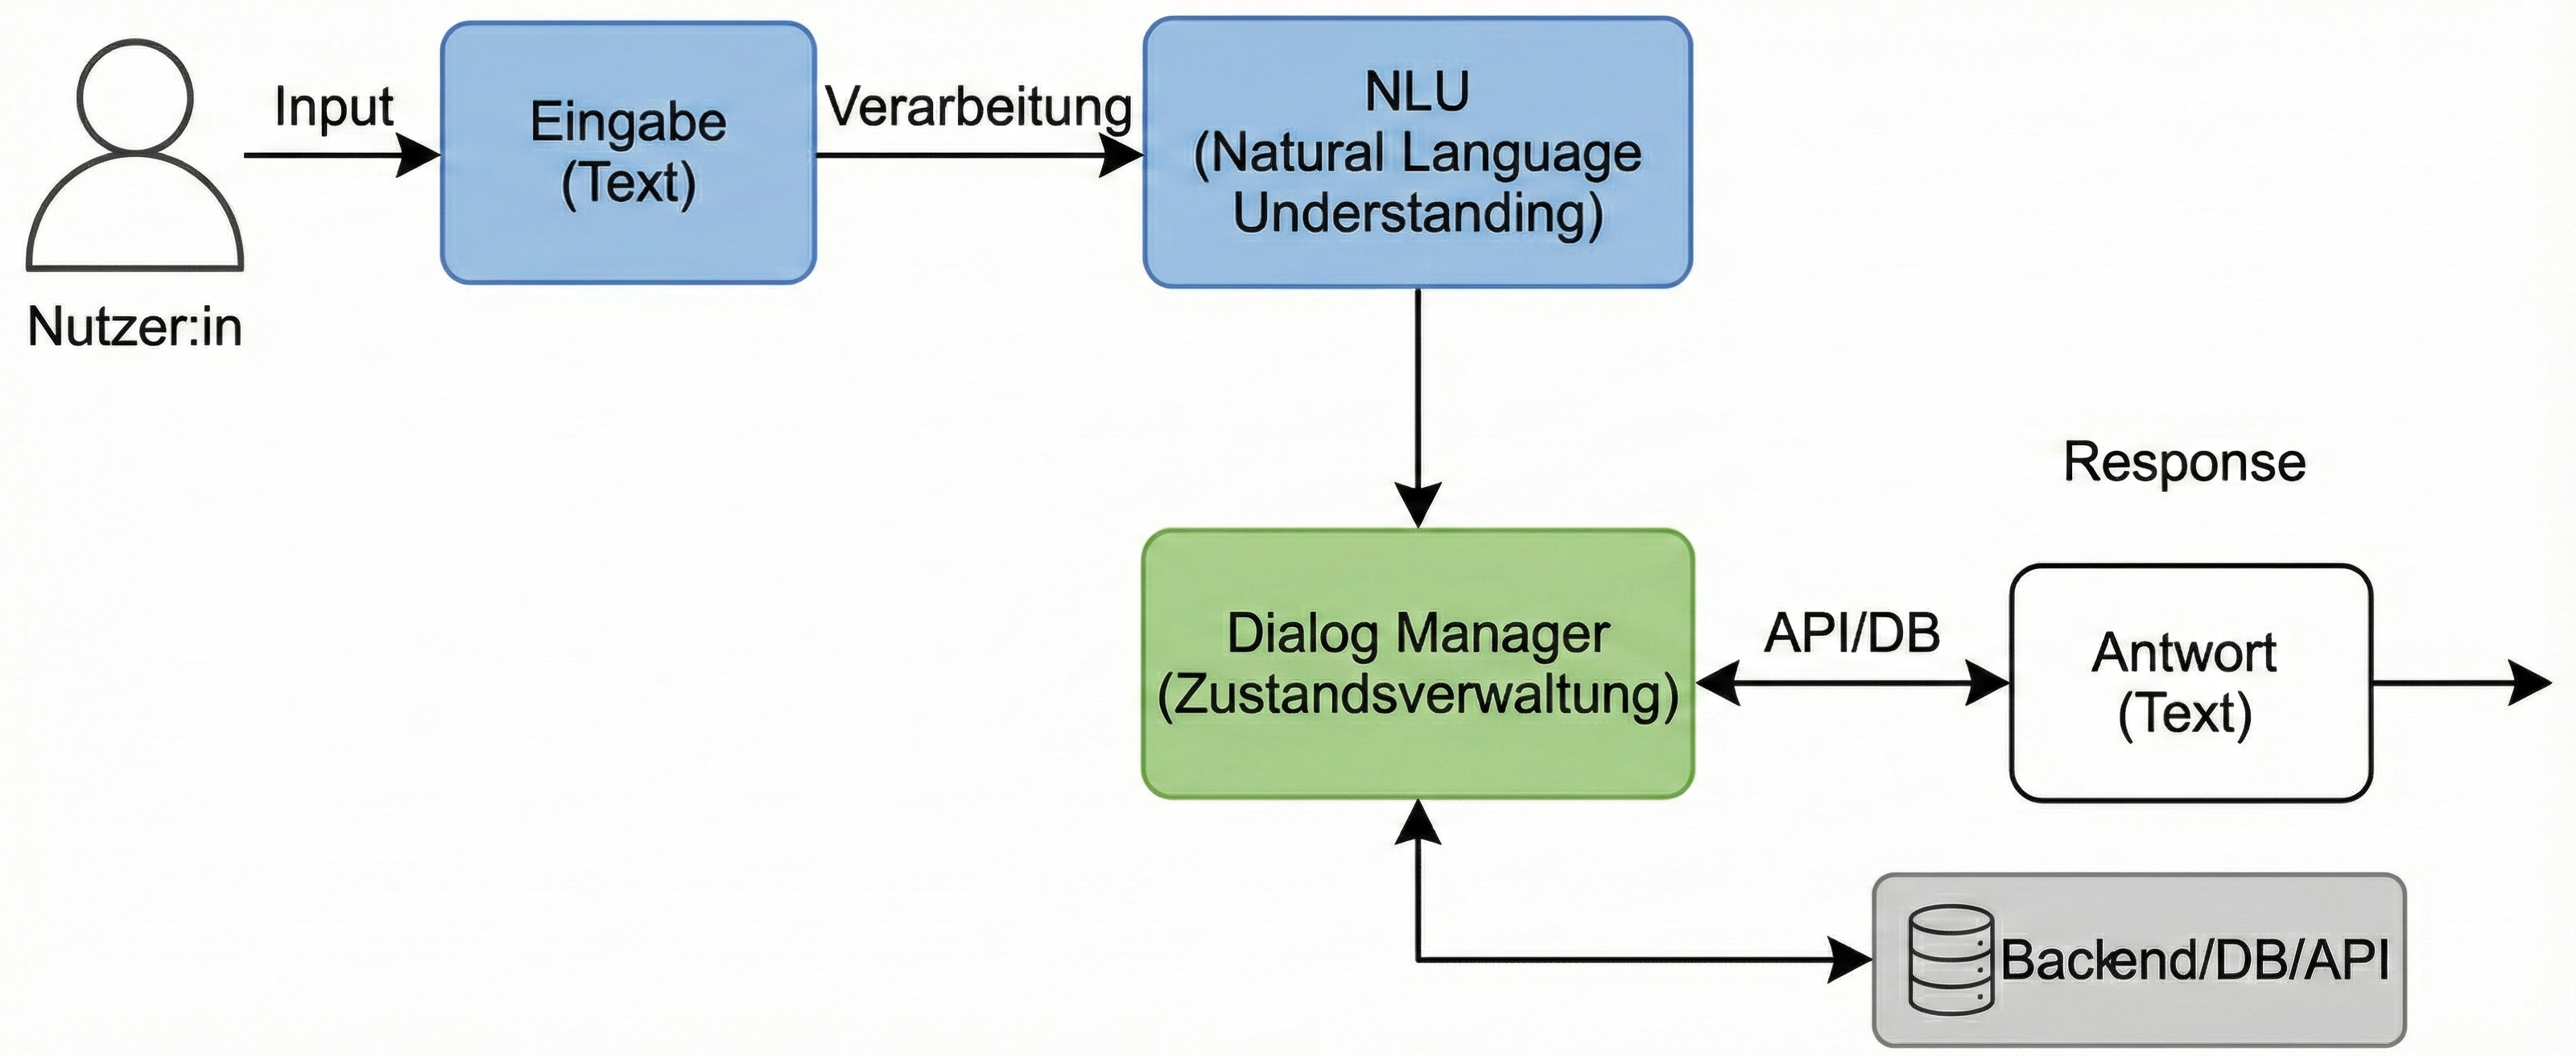
\includegraphics[width=0.92\textwidth]{chatbot_architektur.png}
\caption{Generische Architektur eines dialogbasierten Chatbots.}
\label{fig:chatbot_architektur}
\end{figure}

Zur konsistenten Führung von Dialogen wird häufig ein expliziter Dialogzustand verwaltet. Dieser wird beispielsweise in einer Sitzungsdatenbank gespeichert und ermöglicht es, Kontexte über mehrere Nachrichten hinweg aufrechtzuerhalten. In geschäftskritischen Szenarien werden Chatbots zusätzlich mit Validierungsmechanismen, klar definierten Dialogflüssen und Eskalationspfaden kombiniert. Auf diese Weise lassen sich sowohl eine hohe Nutzerfreundlichkeit als auch die erforderliche Prozesssicherheit gewährleisten.

Im Finanz- und Rechnungswesen werden Chatbots zunehmend zur Unterstützung wiederkehrender und stark strukturierter Aufgaben eingesetzt. Dazu zählen unter anderem die Beantwortung typischer Rückfragen, die Erfassung standardisierter Informationen oder das Anstoßen definierter Geschäftsprozesse. Ein wesentlicher Vorteil dialogbasierter Systeme besteht darin, dass sie über etablierte Kommunikationskanäle wie Messenger-Anwendungen verfügbar sind. Dadurch lassen sie sich ohne umfangreiche Schulungsmaßnahmen in bestehende Arbeitsabläufe integrieren. Die Interaktion verlagert sich hierbei von komplexen Formularoberflächen hin zu einer geführten, schrittweisen Datenerfassung im Dialog \cite{chatbots_finanzprozesse}.

Das in dieser Arbeit vorgestellte System nutzt diese Eigenschaften, indem ein Chatbot als zentrale, dialogbasierte Schnittstelle zur Erfassung von Rechnungs- und Dokumentendaten eingesetzt wird. Der Chatbot führt Nutzerinnen und Nutzer schrittweise durch den Erfassungsprozess, fragt fehlende Informationen gezielt ab und überprüft Eingaben unmittelbar auf Plausibilität. Die dabei gewonnenen strukturierten Daten werden anschließend an cloudbasierte Backend-Dienste übermittelt. Dort werden sie gespeichert, für die automatisierte Dokumentenerzeugung verwendet und in nachgelagerte Prozessschritte integriert. Auf diese Weise wird der Übergang von informeller Kommunikation, etwa einer kurzen Beschreibung der erbrachten Leistung per Text- oder Sprachnachricht, zu formalisierten Verwaltungsprozessen im Rechnungswesen weitgehend automatisiert und ohne Medienbrüche umgesetzt.

Daraus leitet sich für diese Arbeit die Anforderung ab, dass der Chatbot WhatsApp als etablierten Kanal nutzt, einen regelbasierten Dialogzustand mit Sitzungsdatenbank verwaltet und strukturierte Rechnungsdaten sicher extrahiert.




\section{Cloudbasierte Datenhaltung und Integrationen}
\label{sec:cloud-datenhaltung}
Cloudbasierte Datenhaltung bezeichnet die Speicherung von Informationen in extern betriebenen Rechenzentren, auf die über das Internet zugegriffen wird \cite{cloud_grundlagen}. Für kleine Dienstleistungsunternehmen und Einzelunternehmer entfällt dadurch der Bedarf an eigener Serverinfrastruktur, während Daten orts- und geräteunabhängig verfügbar sind. Wartung, Ausfallsicherheit und Skalierung werden weitgehend von spezialisierten Anbietern übernommen, sodass sich die Unternehmen stärker auf ihr Kerngeschäft konzentrieren können.

Ein zentrales Merkmal cloudbasierter Systeme sind standardisierte Programmierschnittstellen. Über solche Web-\glspl{ac:api} können unterschiedliche Anwendungen Daten lesen, schreiben und verarbeiten, ohne direkt auf die zugrunde liegende Infrastruktur zugreifen zu müssen. Web-Frontends, mobile Anwendungen und Automatisierungsdienste nutzen denselben Datenbestand, was Mehrfacherfassungen reduziert und konsistente Informationen in verschiedenen Nutzungskontexten ermöglicht.

Im Rechnungswesen kleiner Unternehmen erlaubt dieser Ansatz die Kombination spezialisierter Dienste statt eines monolithischen Systems. Eine cloudbasierte Datenbank kann etwa Kunden- und Rechnungsinformationen verwalten, während ein separater Speicherdienst für die Ablage von Dokumenten und eine Messaging-Plattform für die Kommunikation mit Nutzenden zuständig sind. Über Integrationslogik im Backend oder in Automatisierungsworkflows werden diese Komponenten zu einem durchgängigen Gesamtsystem verknüpft, in dem Daten zwischen den Diensten ausgetauscht und in unterschiedlichen Oberflächen wiederverwendet werden.

Für das in dieser Arbeit betrachtete Szenario bedeutet dies, dass Stammdaten, Rechnungsinformationen und Verweise auf Dokumente zentral in der Cloud geführt werden, während ergänzende Dienste wie Dokumentengenerierung und Dateispeicherung eigenständig, aber angebunden betrieben werden. Chatbot und Webanwendung greifen auf dieselben Daten zu und stoßen über integrierte Schnittstellen fachliche Prozesse an. Dadurch entsteht eine flexible Architektur, in der einzelne Dienste bei Bedarf ersetzt oder erweitert werden können, ohne die Gesamtstruktur grundlegend ändern zu müssen.





\section{Dokumentengenerierung in der Cloud}
\label{sec:dokumentengenerierung}
Unter Dokumentengenerierung in der Cloud wird die automatisierte Erstellung von Dateien wie Rechnungen, Angeboten oder Verträgen auf Basis digital vorliegender Daten verstanden. Anstatt Dokumente manuell in Textverarbeitungsprogrammen zu erstellen, werden strukturierte Informationen – etwa Kundenstammdaten, Positionslisten oder Zahlungsbedingungen – mit vordefinierten Vorlagen verknüpft. Die eigentliche Erzeugung des Dokuments erfolgt in einer Cloud-Umgebung, sodass keine lokale Bürosoftware erforderlich ist und die Erstellung jederzeit von verschiedenen Endgeräten ausgelöst werden kann.

Technisch basiert dieser Ansatz typischerweise auf Vorlagen, die Layout, Formatierung und feste Textbestandteile enthalten, während variable Inhalte über Platzhalter eingefügt werden.

Eine exemplarische Vorlage mit Platzhaltern ist in \autoref{fig:rechnung_vorlage} dargestellt.

\begin{figure}[H]
\centering
\includegraphics[width=0.85\textwidth]{rechnung_vorlage.png}
\caption{Google Docs Vorlage mit Platzhaltern für automatisierte Rechnungserstellung.}
\label{fig:rechnung_vorlage}
\end{figure}

 Bei der Generierung werden die Platzhalter durch konkrete Werte aus einem Datensystem ersetzt, wodurch aus einer einzigen Vorlage eine Vielzahl individueller Dokumente entstehen kann. Die Ausgabeformate reichen von bearbeitbaren Textdokumenten bis hin zu nicht veränderbaren Formaten wie \gls{ac:pdf}, die sich für den Versand an Kunden und für die revisionsorientierte Ablage eignen. Anpassungen am Erscheinungsbild oder an rechtlichen Pflichtangaben erfolgen zentral an der Vorlage und wirken sich unmittelbar auf alle zukünftigen Dokumente aus.

Die Cloud-Ausführung eröffnet zusätzliche Möglichkeiten der Integration in digitale Geschäftsprozesse. Dokumente können unmittelbar nach ihrer Erstellung automatisiert weiterverarbeitet werden, etwa durch Versand per E-Mail oder Messenger, Speicherung in strukturierten Ordnerhierarchien oder Übergabe an nachgelagerte Systeme wie Buchhaltung oder Dokumentenmanagement. Durch die enge Kopplung mit datenhaltenden Systemen und Workflows lassen sich manuelle Zwischenschritte deutlich reduzieren. Für kleine Unternehmen entsteht so ein durchgängiger Prozess von der Datenerfassung über die Dokumentenerzeugung bis zur Ablage, ohne dass Medienbrüche oder manuelle Formatierungsarbeit erforderlich sind \cite{dokumentengenerierung_cloud, google_docs_mailmerge}.

Für das entwickelte System wird daher eine Google Docs-Vorlage mit Platzhaltern verwendet, die automatisch mit Airtable-Daten befüllt und als PDF in Google Drive revisionssicher abgelegt wird.


\section{Grundlagen moderner Webanwendungen}
\label{sec:webanwendungen}
Moderne Webanwendungen unterscheiden sich deutlich von klassischen, statischen Websites. Während früher hauptsächlich einzelne HTML-Seiten ausgeliefert wurden, handeln aktuelle Anwendungen komplexe Geschäftslogik, dynamische Daten und interaktive Benutzeroberflächen im Browser. Grundlage ist dabei das Client–Server-Modell: Ein Webbrowser fungiert als Client, der über das \gls{ac:http}-Protokoll Anfragen an einen Server sendet. Der Server verarbeitet diese Anfragen, greift bei Bedarf auf Datenquellen zu und liefert strukturierte Antworten zurück, die im Frontend dargestellt oder weiterverarbeitet werden.

Auf der Client-Seite kommen typischerweise JavaScript-Frameworks zum Einsatz, die Single-Page-Applications (\gls{ac:spa}) ermöglichen. In einer \gls{ac:spa} wird die Benutzeroberfläche nicht bei jedem Seitenwechsel vollständig neu geladen, sondern dynamisch im Browser aktualisiert. Daten werden über asynchrone Anfragen an serverseitige Schnittstellen geladen und in Komponenten gerendert. Dieses Architekturprinzip erlaubt reaktionsschnelle Oberflächen, die sich in ihrer Bedienung eher wie klassische Desktop-Anwendungen verhalten und komplexe Interaktionen, etwa Tabellen mit Filter- und Sortierfunktionen, komfortabel abbilden \cite{webanwendungen_spa}.

Die serverseitige Ebene moderner Webanwendungen stellt meist klar definierte Programmierschnittstellen bereit, häufig in Form von \gls{ac:rest}- oder JSON-basierten \gls{ac:http}-\glspl{ac:api}. Darüber werden fachliche Operationen wie das Lesen, Anlegen oder Aktualisieren von Datensätzen kapsuliert. Ergänzend gewinnen serverlose Architekturen und sogenannte Edge Functions an Bedeutung, bei denen einzelne Funktionsbausteine ereignisgesteuert und skalierbar in einer Cloud-Umgebung ausgeführt werden. Sicherheitsmechanismen wie Authentifizierung und Autorisierung, Transportverschlüsselung sowie rollenbasierte Zugriffskonzepte sind integraler Bestandteil solcher Anwendungen und sorgen dafür, dass sensible Daten nur von berechtigten Nutzenden eingesehen oder verändert werden können.

Die ClientHub-Web-App nutzt dieses SPA-Prinzip mit React, TypeScript und Edge Functions für die strukturierte Darstellung von Kunden- und Rechnungsdaten aus Airtable sowie den Zugriff auf Drive-Dokumente.
